\section{Постановка задачі техніко-економічного аналізу}
У роботі застосовується метод ФВА для проведення техніко-економічного аналізу розробки.

Відповідно цьому варто обирати і систему показників якості програмного продукту. 

Технічні вимоги до продукту наступні:
\begin{itemize}
	\item програмний продукт повинен функціонувати на персональних комп'ю\-терах зі стандартним набором компонент;
	\item забезпечувати високу швидкість обробки великих об'ємів даних у реальному часі;
	\item забезпечувати зручність і простоту взаємодії з користувачем або з розробником програмного забезпечення у випадку використання його як модуля;
	\item передбачати мінімальні витрати на впровадження програмного продукту.
\end{itemize}

\subsection{Обґрунтування функцій програмного продукту}
Головна функція $F_0$ – розробка програмного продукту, який аналізує процес за вхідними даними та будує його модель для подальшого прогнозування. Виходячи з конкретної мети, можна виділити наступні основні функції ПП:
\begin{description}
	\item[$F_1$] вибір мови програмування;
	\item[$F_2$] вибір оптимальної бібліотеки для математичних обчислень;
	\item[$F_3$] інтерфейс користувача.
\end{description}


Кожна з основних функцій може мати декілька варіантів реалізації.
\begin{itemize}
\item Функція F1 :
	\begin{enumerate}
		\item мова програмування C++;
		\item  мова програмування Python.
	\end{enumerate}
\item Функція F2:
	\begin{enumerate}
		\item STL;
		\item boost::ublas;
		\item Numpy/Scipy.
	\end{enumerate}
\item Функція F3:
	\begin{enumerate}
		\item консольний інтерфейс користувача;
		\item графічний інтерфейс користувача, створений за технологією Qt.
	\end{enumerate}
\end{itemize}

\subsection{Варіанти реалізації основних функцій}
Варіанти реалізації основних функцій наведені у морфологічній карті системи (\imref{fig:economics_morph}). На основі цієї карти побудовано позитивно-негативну матрицю варіантів основних функцій (Таблиця~\ref{tab:economics_positive_negative_matrix}). 

\begin{figure}
	\centering
	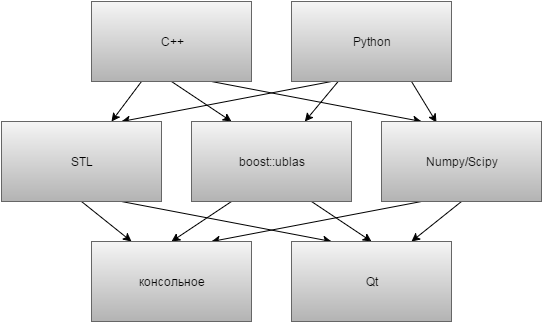
\includegraphics[width=0.7\linewidth]{chapter_Economics/img/map}
	\caption{Морфологічна карта}
	\label{fig:economics_morph}
\end{figure}


Морфологічна карта відражає всі можливі комбінації варіантів реалізації функцій, які складають повну множину варіантів ПП.

\begin{table}[tbp]
	\caption{Позитивно-негативна матриця}
	\centering
\begin{tabular}{|p{0.12\textwidth}|p{0.13\textwidth}|p{0.3\textwidth}|p{0.3\textwidth}|}\hline
	Основні функції & Варіанти реалізації & Переваги &  Недоліки \\ 
\hline
\multirow{2}{*}{F1}	& А &  Максимальна швидкість роботи, кросплатформений, краща підтримка
					& Вищий поріг входу, менша швидкість розробки\\ 
	 \cline{2-4} 
					& Б & простіший у використанні, вища швидкість розробки
				    & Нижча швидкодія\\
\hline
\multirow{3}{*}{F2} & А &  Безкоштовний, кросплатформений продукт, велика кількість якісної документації, краща підтримка
					& Високий поріг входу, велика кількість речей, що потребують обережної поведінки з ними\\ 
	\cline{2-4}         
					& Б & Велика бібліотека готових функцій
					& Потребує підключення додаткових модулів\\
	\cline{2-4}         
					& В & Велика бібліотека готових функцій, що легкі у використанні 
					& Менша швидкодія, при роботі з мови Python необхідно уникати циклів для оптимізації\\
\hline
\multirow{2}{*}{F3} & А & Простота роботи, гнучкість інтерфейсу, швидкість розробки, кросплатформеність
					& Високий поріг входу, складність і незрозумілість побудови інтерактивної системи \\
	\cline{2-4}
					& Б & Низький поріг входу, кросплатформеність, висока швидкість роботи і розробки
					& Тільки для С++ та врапперів, більша складність розробки\\
\hline
	\end{tabular}
	\label{tab:economics_positive_negative_matrix}
\end{table}

На основі аналізу позитивно-негативної матриці робимо висновок, що при розробці програмного продукту деякі варіанти реалізації функцій варто відкинути, тому, що вони не відповідають поставленим перед програмним продуктом задачам. Ці варіанти відзначені у морфологічній карті.
\subsubsection{Функція $F_1$}
Відкидаємо варіант б) через те, що для даного продукту дуже важливо зберігати велику швидкодію, хоча це потребує більшої професійності при побудові додатку.
\subsubsection{Функція $F_2$}
\label{subsub:economics_f2}
Оскільки програмний продукт створюється за допомогою C++, логічно вибирати бібліотеку для роботи з зображеннями, що первісно написана для мов C/C++. Хоча варіант використання бібліотек Numpy/Scipy залишається можливим, він більш складний у побудові і буде мати меншу швидкодію внаслідок додаткової передачі даних через враппер Python.

Використання бібліотеки boost є досить прийнятним, але бібліотеки STL, що вбудована в C++, цілком достатньо для проведення разрахунків, тому нема сенсу підключати додаткові бібліотеки з аналогічним функціоналом.
\subsubsection{Функція $F_3$}
Вважаємо варіанти А і Б гідними розгляду. Кожен має свої переваги та недоліки.

Таким чином, будемо розглядати такі варіанти реалізації ПП: 
\newcommand{\econf}[2]{F_{#1\text{#2} } }
\begin{enumerate}
	\item $\econf{1}{а}$ – $\econf{2}{а}$ – $\econf{3}{а}$
	\item $\econf{1}{а}$ – $\econf{2}{а}$ – $\econf{3}{б}$
\end{enumerate}
Для оцінювання якості розглянутих функцій обрана система параметрів, описана нижче.